\newpage
\section{Ecuaciones Diferenciales Ordinarias}
 \subsection{Método de Euler}
 \subsection{Método del salto de la rana}
  \subsubsection{Motivación}
   Si bien el método de Euler es un approach simple y familiar (pero no muy estable) a la resolución numérica 
   de EDO's, \textbf{físicamente} plantea un problema importante: \textbf{no conserva la energía del sistema}. Un rápido cálculo nos muestra esto:\\
   \subsubsubsectionanum{Ejemplo}
    Para un sistema masa-resorte colgando, se puede mostrar que \textbf{energía total} del sistema\footnote{Se ha considerado $m=1$.} es de la forma:
   \begin{equation}
     E(t) = \frac{1}{2}v^2 + \frac{1}{2}\omega^2 \left( y + \frac{g}{\omega^2} \right)^2. \label{eq:ener_euler}
  \end{equation}
  Luego, bajo el método de Euler, la energía en tiempos discretos es:

  \begin{align*}
  E_{n+1} &= \frac{1}{2} v_{n+1}^2 + \frac{1}{2} \omega^2 \left( y_{n+1} + \frac{g}{\omega^2} \right)^2 \,, \\
  &= \frac{1}{2} \left[ v_n - h(\omega^2 y_n + g) \right]^2 + \frac{1}{2} \omega^2 \left[ y_n + h v_n + \frac{g}{\omega^2} \right]^2 \,, \\
  &= (1 + \omega^2 h^2) \left[ \frac{1}{2} v_n^2 + \frac{1}{2} \omega^2 \left( y_n + \frac{g}{\omega^2} \right)^2 \right] \,, \\
  &= (1 + \omega^2 h^2) E_n \,.
  \end{align*}
Es decir, el método de Euler no conserva la energía pues $E_{n+1} > E_n$ para todo $n$. Puede ver esto también modelando la ecuación \eqref{eq:ener_euler}, o realizando un gráfico de rapidez versus posición (una especie de espacio de fases) mientras evoluciona el tiempo (ver figura \ref{fig:dos_graficos}). El hecho que la trayectoria no sea cerrada en el espacio de fases es consecuencia directa de la pérdida de energía. 
\begin{figure}[htbp]
    \centering
    \begin{minipage}{0.48\textwidth}
        \centering
        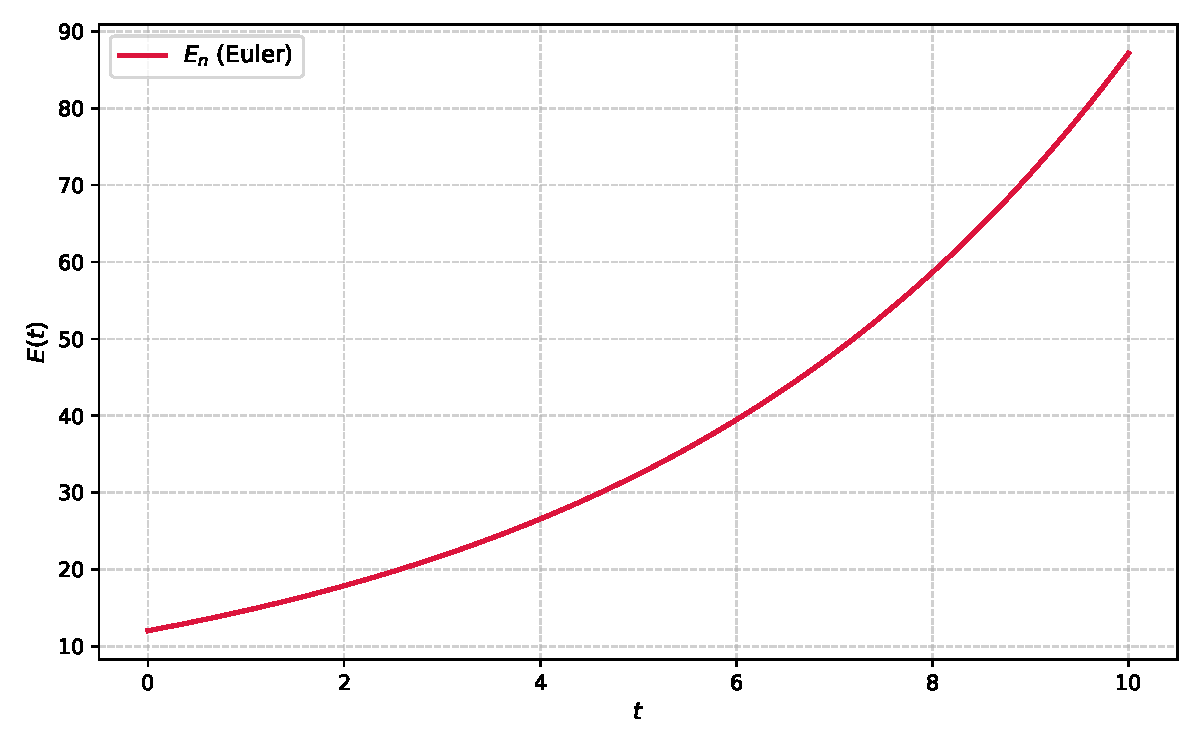
\includegraphics[width=\textwidth]{img/ejemplos/E(t).pdf}
    \end{minipage}
    \hfill
    \begin{minipage}{0.48\textwidth}
        \centering
        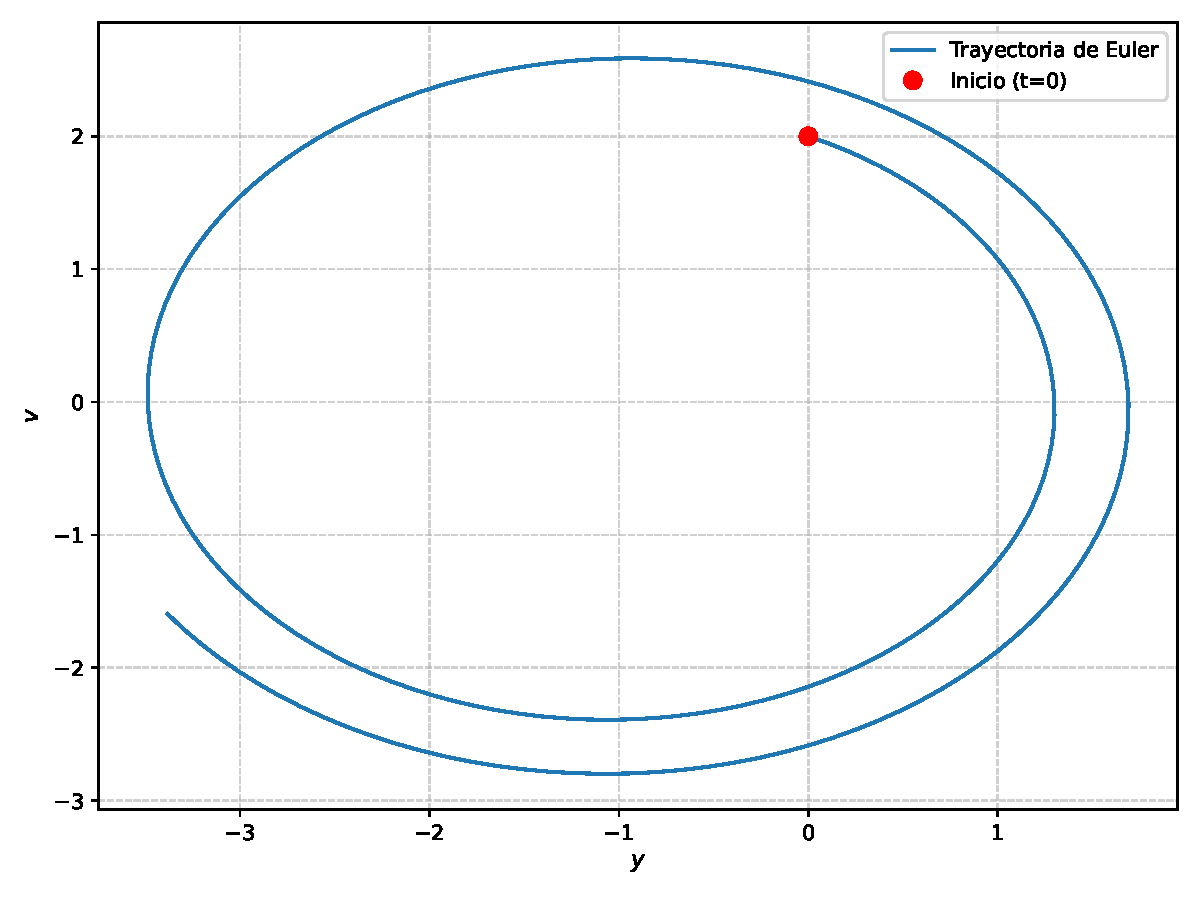
\includegraphics[width=\textwidth]{img/ejemplos/phase_space_Euler.pdf}
    \end{minipage}
    \caption{Gráficos de energía y espacio de fases para el método de Euler.}
    \label{fig:dos_graficos}
\end{figure}

